\documentclass{article}

\usepackage[a4paper, total={6in, 8in}]{geometry}

\usepackage{amsmath}
\usepackage{amsfonts}
\usepackage{amssymb}
\usepackage[T1, T2A]{fontenc}
\usepackage[utf8]{inputenc}
\usepackage[english, russian]{babel}
\usepackage{graphics}
\usepackage{graphicx}
\usepackage{makecell}

\geometry{
 a4paper,
 total={170mm,257mm},
 left=20mm,
 top=20mm,
 }

\author{Александр Валентинов}
\title{Лабораторная работа 3.4.1}

\begin{document}
   \subsection*{Работа 3.4.1}
   \section*{Диа- и парамагнетики}
   \paragraph*{Цель работы:} измерение магнитной восприимчивости диа- и парамагнитного образцов.
   \paragraph*{В работе используются:} электромагнит, аналитические весы, милливеберметр, амперметр постоянного тока, реостат, образцы.
   \subsubsection*{Экспериментальная установка}
   \begin{figure}[h]
   \centering
   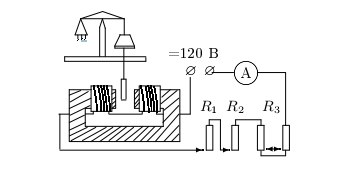
\includegraphics[width=8cm]{fig1.jpg} 
   \caption{Схема экспериментальной установки} 
   \label{fig.1} 
   \end{figure}
   \subparagraph*{Обработка результатов}
   Построим график $B(I)$ (Рисунок \ref{plot.1}, таблица \ref{table.1}), чтобы определять величину магнитной индукции по току. Будем считать $B$ по формуле
   \[ B = \frac{\Phi}{SN},~~ \sigma_b = \sqrt{\left(\frac{\sigma_\Phi}{SN}\right)^2 + \left( \frac{\Phi}{SN} \frac{\sigma_{SN}}{SN} \right)^2}. \]
   \begin{figure}[h]
   \centering
   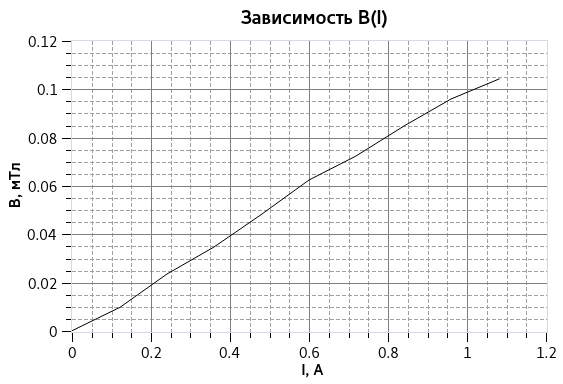
\includegraphics[width=16cm]{plot1.png} 
   \caption{Зависимость $B(I)$} 
   \label{plot.1} 
   \end{figure}
   \begin{table} 
 \caption{Зависимость для RC-цепи}
 \label{RCtable}
\begin{center}
\begin{tabular}{|*{4}{r|}}
\hline 
$\psi$ & $\tan \psi$ & $\sigma_{\tan_\psi}$ & $1 / (\Omega C R_\Sigma)$ \\ \hline 
 1.51 & 16   & 1    & 25.7  \\ \hline 
 1.26 & 3.1  & 0.2  & 2.83  \\ \hline 
 1.01 & 1.6  & 0.1  & 1.65  \\ \hline 
 0.75 & 0.94 & 0.09 & 0.93  \\ \hline 
 0.50 & 0.55 & 0.07 & 0.566 \\ \hline 
 0.25 & 0.26 & 0.07 & 0.260 \\ \hline 
 0.00 & 0.00 & 0.06 & 0.099 \\ \hline 
 \end{tabular}
\end{center} 
\end{table} 

   Найдем зависимость $\Delta P(B^2)$, чтобы найти магнитную восприимчивость веществ.
   \[ \sigma_{B^2} = 2B\sigma_B \]

   \[ k_{Al} = \left(-\frac{\chi s}{2\mu_0}\right)_{Al} =  -4.30 \pm 0.08 \frac{\text{кг}\cdot\text{м}}{\text{с}^2 \cdot \text{мТл}^2},~~  k_{Cu} = 2.24 \pm 0.08 \frac{\text{кг}\cdot\text{м}}{\text{с}^2 \cdot \text{мТл}^2} \]

   \[ \chi =  -\frac{2k\mu_0}{s},~~ \sigma_\chi = \frac{2k\mu_0}{s^2}\sigma_s,~~ s = \pi \frac{d^2}{4},~~ \sigma_s = \frac{\pi d \sigma_d}{2} \]

   \[ \chi_{Al} = (0.16 \pm 0.03) \cdot 10^{-6},~~ \chi_{Cu} = (-0.073 \pm 0.007) \cdot 10^{-6} \]
   Полученные значения сходятся с табличными по порядку величины.
   \begin{table} 
 \caption{Table2}
\begin{tabular}{|*{8}{c|}}
\hline 
I & Ex0.3 & Ex0.45 & Ex0.5 & Ex0.65 & Ex0.8 & Ex0.95 & Ex-0.95\\ \hline 
17.2 & 0 & 0 & 0 & 0 & 0 & 0 & 0 \\ \hline 
 181.9 & 0.051 & 0.072 & 0.084 & 0.109 & 0.129 & 0.159 & 0.166 \\ \hline 
 378.1 & 0.103 & 0.151 & 0.169 & 0.218 & 0.266 & 0.319 & 0.328 \\ \hline 
 571.8 & 0.151 & 0.224 & 0.251 & 0.322 & 0.396 & 0.472 & 0.496 \\ \hline 
 730.7 & 0.195 & 0.288 & 0.323 & 0.417 & 0.508 & 0.605 & 0.64 \\ \hline 
 854.4 & 0.228 & 0.336 & 0.378 & 0.487 & 0.595 & 0.71 & 0.75 \\ \hline 
 934.9 & 0.251 & 0.368 & 0.418 & 0.535 & 0.655 & 0.781 & 0.831 \\ \hline 
 1,003 & 0.269 & 0.394 & 0.446 & 0.569 & 0.698 & 0.83 & 0.884 \\ \hline 
 \end{tabular} 
\end{table} 

   \paragraph*{Вывод:} В ходе работы мы нашли магнитные восприимчивости алюминия и меди.
   \begin{figure}[h]
   \centering
   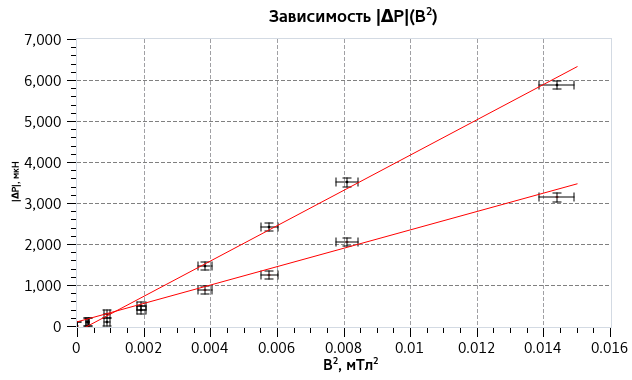
\includegraphics[width=12cm]{plot2.png} 
   \caption{Зависимость $|\Delta P|(B^2)$} 
   \label{plot.2} 
   \end{figure}
\end{document}
